\section{Background Subtraction: autobk algorithm}


\begin{frame} \frametitle{Background Subtraction: $\mu_0(E)$}

\begin{cenpage}{130mm}

  \[ \chi(E) = \frac{\mu(E) - \mu_0(E)}{\Delta \mu_0(E_0)} \]

\vmm
We don't know ${\mu_0(E)}$, so use a {\BlueEmph{spline}}: a smooth, adjustable function.

\vmm

This could be dangerous -- a flexible enough spline would remove all the XAFS.

\vmm
\pause

The {\autobk} method in {\larch} chooses a background spline for $\mu_0(E)$ to

\begin{center}
  \begin{postitbox}{55mm}
    {\RedEmph{minimize the low-$R$ components of $\chi$}}
  \end{postitbox}
\end{center}

\begin{enumerate}
  \item Spline parameters for $\mu_0(E)$ are guessed.
  \item $\chi(k)$ is Fourier Transformed to $\chi(R)$.,
  \item Spline parameters optimized so that $\chi(R)$ below \feffc{R_{\rm bkg}} is minimized.
  \item Note that $\chi(R)$ above \feffc{R_{\rm bkg}} is completely ignored!
\end{enumerate}


\vmm  \hrule \vmm

Most important parameters:

\begin{enumerate}
\item \feffc{R_{\rm bkg}}: $R$ below which $\chi(R)$ is reduced.
\item {\Red{$k$-weight}}:  used for Fourier transform:   use 1, or 2.
\item \feffc{E_0}:         May need to adjust for initial guess (max of $d\mu/dE$).
\end{enumerate}

\end{cenpage}
\end{frame}


\begin{frame} \frametitle{Background Subtraction in {\xasviewer} }

  \begin{cenpage}{130mm}

Effect of \feffc{R_{\rm bkg}}  on XAFS $\chi(k)$ and $\chi(R)$:

\begin{tabular}{ll}
  \begin{minipage}{65mm}
    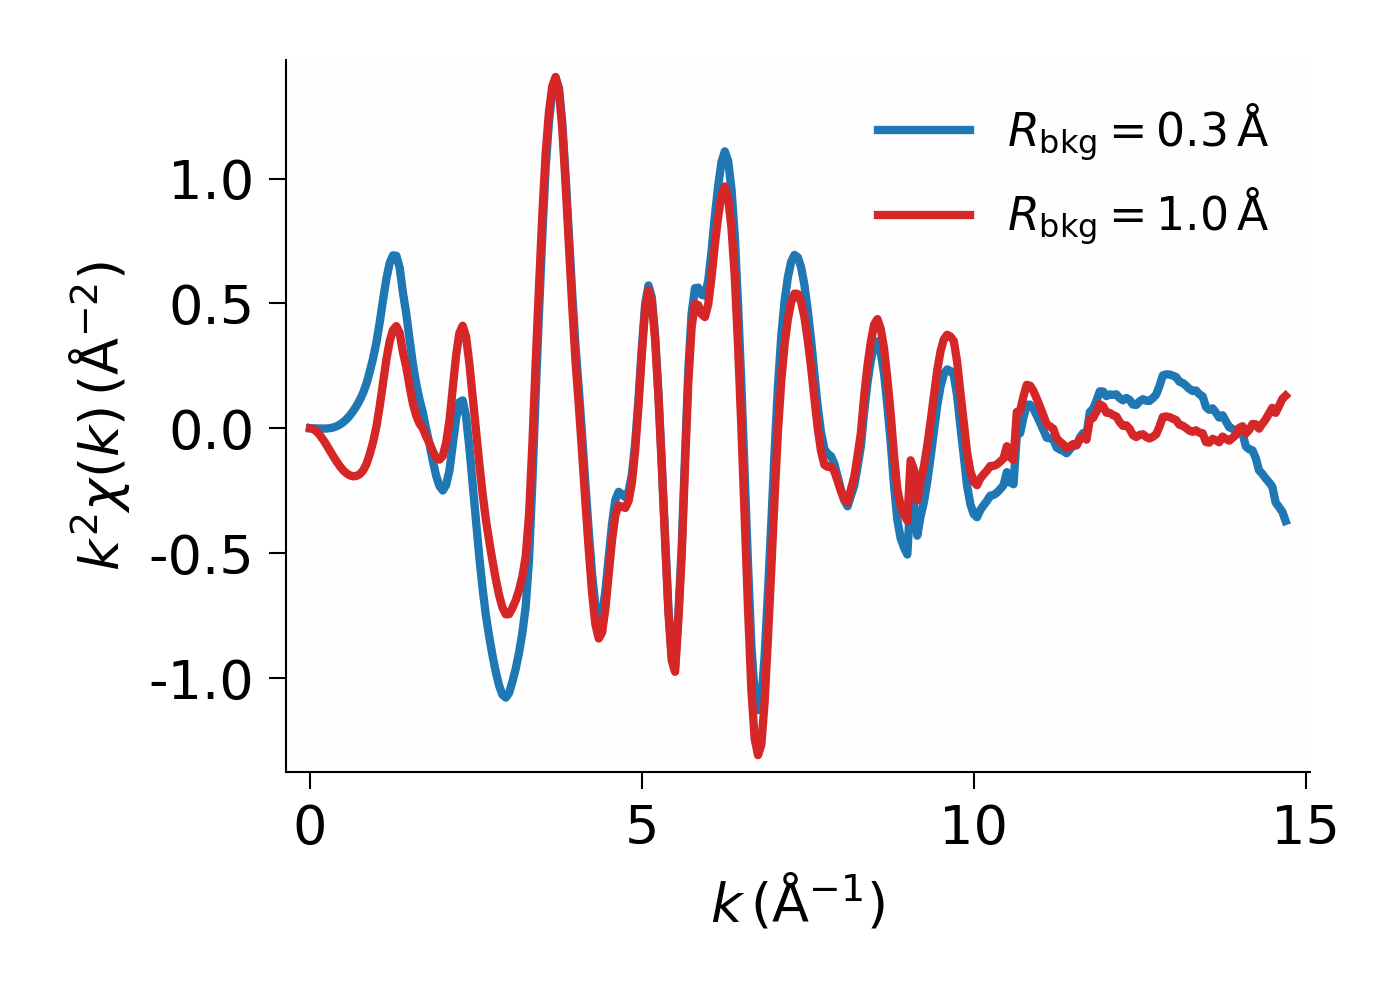
\includegraphics[width=60mm]{figs/experiment/bkg_ksp1}
  \end{minipage} &
  \begin{minipage}{65mm}
    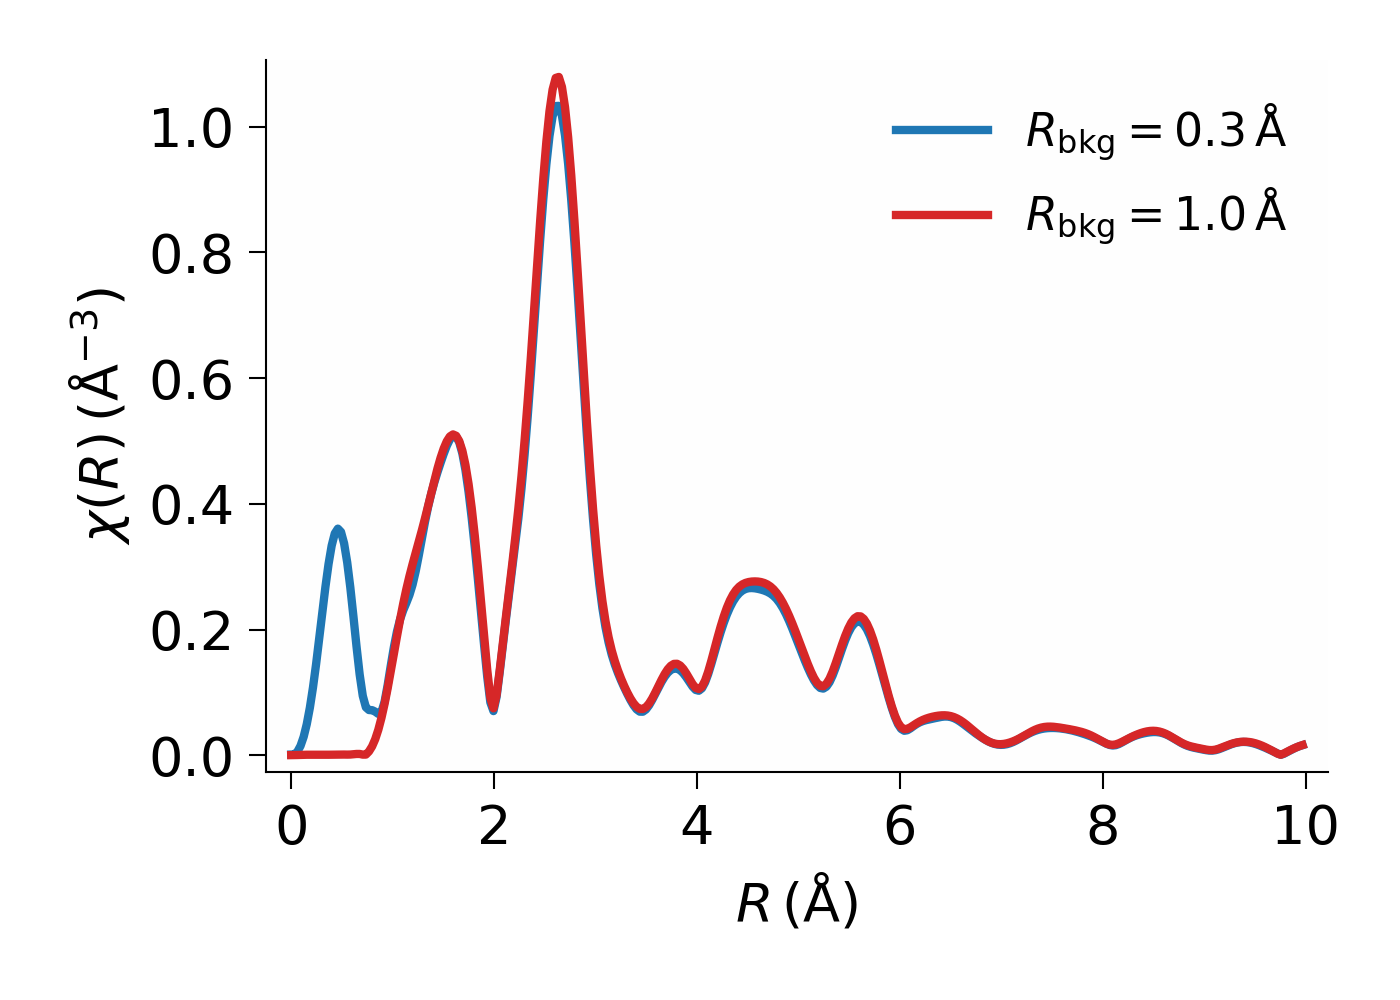
\includegraphics[width=60mm]{figs/experiment/bkg_rsp1}
  \end{minipage} \\
  \begin{minipage}{55mm}
    $\chi(k)$ for FeO with
    $R_{\rm bkg}=0.1\, \rm \AA$ \\
    (stiff spline)  and $R_{\rm bkg}=1.0\, \rm \AA$.
  \end{minipage} &
  \begin{minipage}{55mm}
    $\chi(R)$ for FeO with
    $R_{\rm bkg}=0.1\, \rm \AA$ \\
    (stiff spline)   and  $R_{\rm bkg}=1.0\, \rm \AA$.
  \end{minipage} \\
\end{tabular}

\vmm \pause \vmm\vmm

Rules of thumb:

\begin{postitbox}{76mm}
  Use  $R_{\rm bkg}=1.0\, \rm \AA$ or half the near-neighbor distance.
\end{postitbox}

\begin{postitbox}{76mm}
  Don't spend too much time on background subtraction.
\end{postitbox}

\end{cenpage}

\end{frame}


\begin{frame} \frametitle{Background Subtraction in {\xasviewer}  }


  \begin{cenpage}{130mm}


Don't make \feffc{R_{\rm bkg}} too big!

\begin{tabular}{ll}
  \begin{minipage}{65mm}
    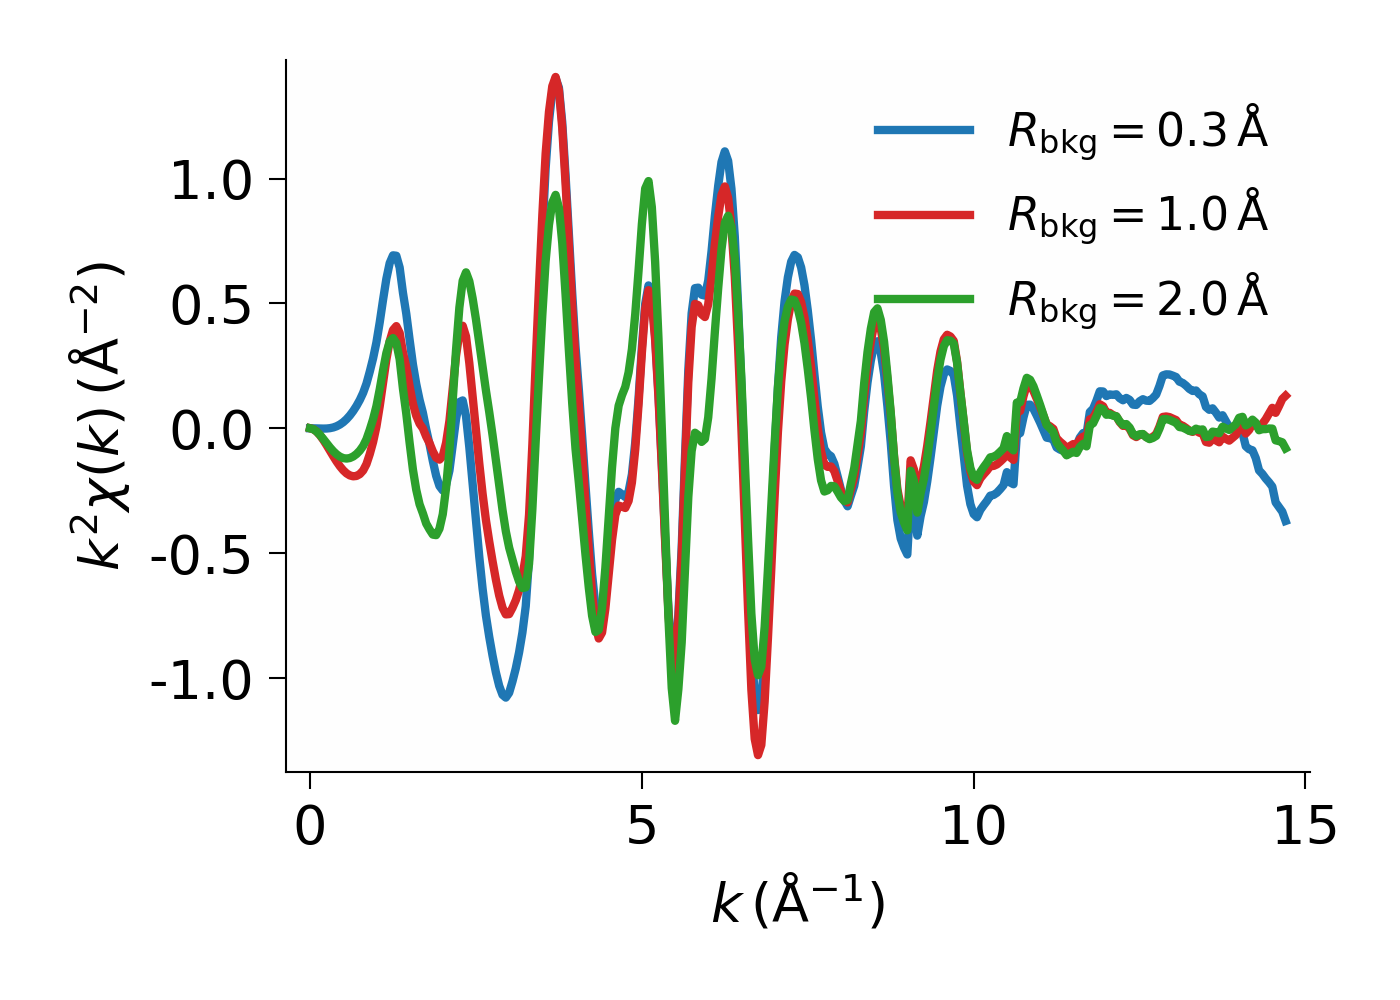
\includegraphics[width=60mm]{figs/experiment/bkg_ksp2}
  \end{minipage} &
  \begin{minipage}{55mm}
    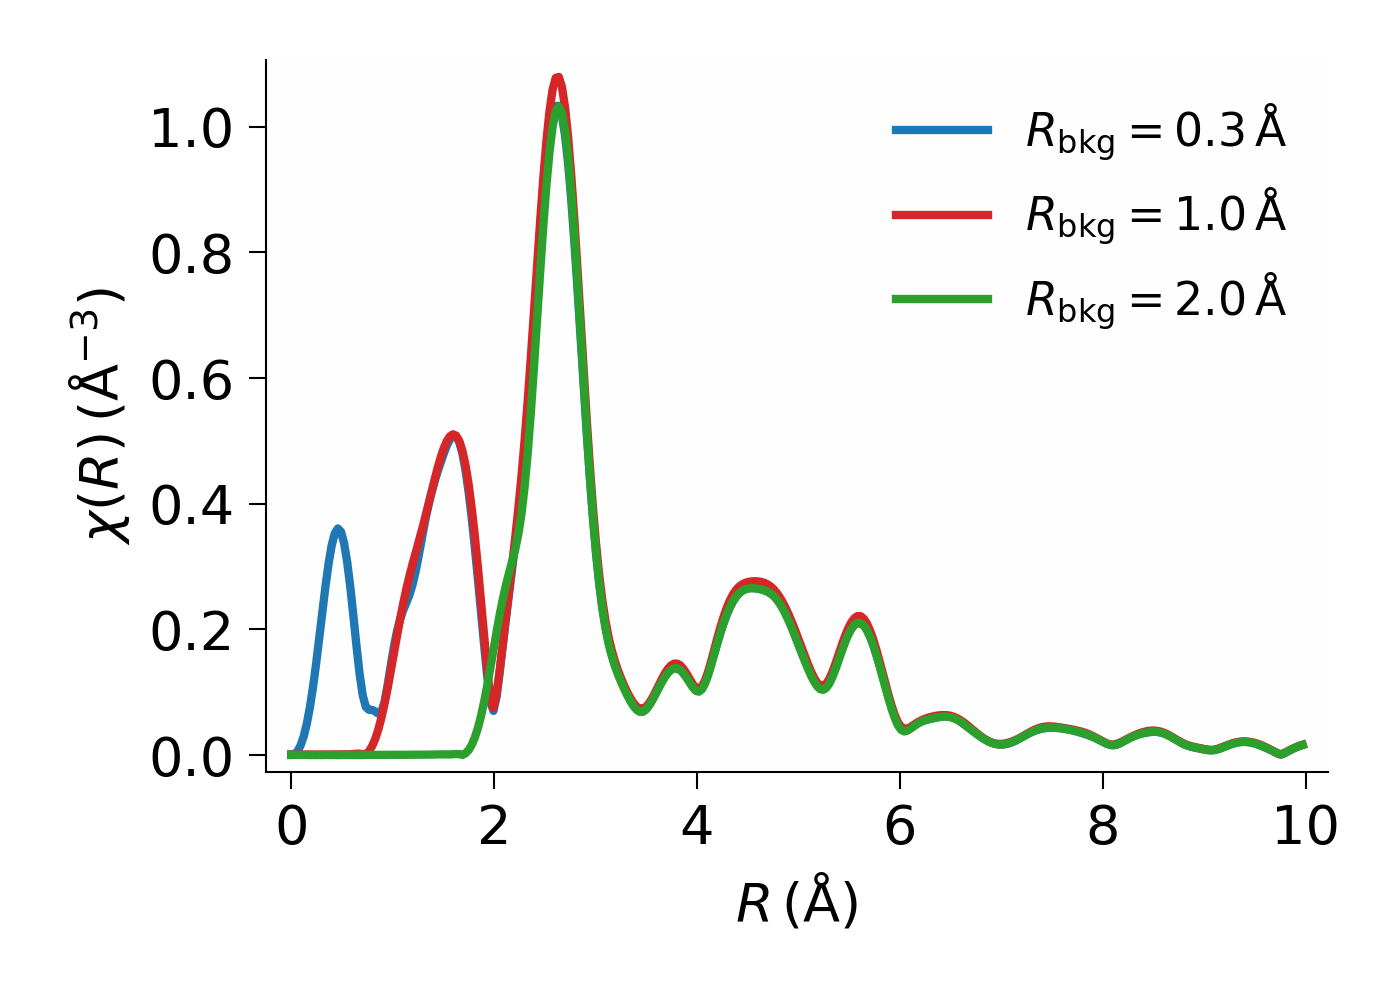
\includegraphics[width=60mm]{figs/experiment/bkg_rsp2}
  \end{minipage} \\
  \begin{minipage}{55mm}
    $\chi(k)$ for FeO with $R_{\rm bkg}=2.0\, \rm \AA$
  \end{minipage} &
  \begin{minipage}{55mm}
    $\chi(R)$ for FeO with $R_{\rm bkg}=2.0\, \rm \AA$  Note: we have
    removed the first shell!!

  \end{minipage} \\
\end{tabular}

\vmm

    \vmm
    Having $R_{\rm bkg}$ too big is the most important thing to avoid.

    \vmm

    $R_{\rm bkg}$  that's a little bit small  and gives a small peak at
    very low $R$ is not that big of a problem.

    \end{cenpage}
\vfill


\end{frame}
